% \documentclass{easychair}
\documentclass[EPiC]{easychair}
%\documentclass[EPiCempty]{easychair}
%\documentclass[debug]{easychair}
%\documentclass[verbose]{easychair}
%\documentclass[notimes]{easychair}
%\documentclass[withtimes]{easychair}
%\documentclass[a4paper]{easychair}
%\documentclass[letterpaper]{easychair}

\usepackage{doc}
\usepackage{float}
\usepackage{amssymb}

\newenvironment{packed_itemize}{
\vspace*{-0.5em}
\begin{itemize}
  \setlength{\partopsep}{0pt}
  \setlength{\itemsep}{1pt}
  \setlength{\parskip}{0pt}
  \setlength{\parsep}{0pt}
}{\end{itemize}}

\newenvironment{packed_enumerate}{
\vspace*{-0.5em}
\begin{enumerate}
  \setlength{\partopsep}{0pt}
  \setlength{\itemsep}{1pt}
  \setlength{\parskip}{0pt}
  \setlength{\parsep}{0pt}
}{\end{enumerate}}

% use this if you have a long article and want to create an index
% \usepackage{makeidx}

% In order to save space or manage large tables or figures in a
% landcape-like text, you can use the rotating and pdflscape
% packages. Uncomment the desired from the below.
% \usepackage{rotating}
% \usepackage{pdflscape}

% Make sure to include the slash at the end of the path name
\graphicspath{ {./figures/} }

% Macros
\DeclareMathOperator*{\argmaxA}{arg\,max} % Jan Hlavacek - argmax function

%\makeindex

%% Front Matter
%%
% Regular title as in the article class.
%
\title{Evaluation of Axiom Selection Techniques}
% \thanks{Other people who contributed to this document include Maria Voronkov
%   (Imperial College and EasyChair) and Graham Gough (The University of
%   Manchester).}}

% Authors are joined by \and. Their affiliations are given by \inst, which indexes
% into the list defined using \institute
%
\author{
Qinghua Liu\inst{1}
 \and
Zishi Wu\inst{2}
 \and
Zihao Wang\inst{2}
 \and
Geoff Sutcliffe\inst{2}
% \thanks{Did numerous tests and provided a lot of suggestions}
}

% Institutes for affiliations are also joined by \and,
\institute{
%  School of Information Science and Technology, 
  Southwest Jiaotong University, China, \email{qhliu@my.swjtu.edu.cn}
\and
   University of Miami, USA, \email{zishi@cs.miami.edu,zxw526@miami.edu,geoff@cs.miami.edu}
 }

%  \authorrunning{} has to be set for the shorter version of the authors' names;
% otherwise a warning will be rendered in the running heads. When processed by
% EasyChair, this command is mandatory: a document without \authorrunning
% will be rejected by EasyChair

\authorrunning{Liu, Wu, Wang, Sutcliffe}

% \titlerunning{} has to be set to either the main title or its shorter
% version for the running heads. When processed by
% EasyChair, this command is mandatory: a document without \titlerunning
% will be rejected by EasyChair
\titlerunning{Evaluation of Axiom Selection Techniques}

\begin{document}

\maketitle
%------------------------------------------------------------------------------
\begin{abstract}
``Large theory'' problems in Automated Theorem Proving (ATP) have been
defined as having {\em many functions and predicates, and many axioms of
which only a few are required for the proof of a theorem}.
One key to solving large theory problems is selecting a subset of the axioms
that is adequate for finding a proof.
The main contribution of this paper is metrics for evaluating axiom selection 
techniques without having to run an ATP system on the problem formed from 
the selected axioms and the problem's conjecture.
This paper additionally presents three new axiom selection techniques.
The new techniques, and the axiom selection in the Vampire ATP 
system, are evaluated using the metrics.
\end{abstract}
%------------------------------------------------------------------------------
\section{Introduction}
\label{Introduction}

``Large theory'' problems in Automated Theorem Proving (ATP) have been 
defined \cite{Sut20-CASC} as having {\em many functions and predicates, and 
many axioms of which only a few are required for the proof of a theorem}.
Large theory problems are often found in corpora that contain very many
problems, e.g., the MPTP2078 corpus \cite{AH+14}, the Mizar 40 corpus
\cite{KU15-M40}, and the GRUNGE corpus \cite{BG+19}.
Large theory problems present challenges to ATP systems, mainly because of the
large search space generated by the large number of axioms.
Thus, one key to solving large theory problems is selecting a subset of the 
axioms that is adequate for finding a proof. 
There has been significant and successful research on this topic, e.g.,
\cite{PSZG04,SP07,MP09,KC+10,HV11,Kv+12,AH+14,GK15,PU18}.
Many techniques are based on the occurrences of symbols in the formulae,
e.g., the SInE method \cite{HV11} and its derivatives. 
The fact that large theory problems often occur in large corpora makes the
application of machine learning techniques \cite{KB14} viable, e.g., as 
in the MaLARea system \cite{US+08}.

Evaluation of axiom selection techniques is typically done by:
\begin{packed_enumerate}
\item Choosing a corpus of large theory problems that are known to be theorems.
\item For each problem in the corpus, selecting a subset of the problem's
      axioms.
\item Running an ATP system on the reduced problem formed from the selected 
      axioms and the problem's conjecture.
\end{packed_enumerate}
In the third step of this process, a proof indicates an adequate selection
(the quality of which can then be evaluated), and a countermodel indicates 
an inadequate selection. 
As the development of axiom selection techniques progresses, this approach 
requires repeating steps 2 and 3 to evaluate progress.
Evaluation needs to be done on large corpora, making this a time consuming 
process.
As a consequence, to move things along faster, it is often necessary to impose 
a small time limit on each ATP system run.
Time limits (and other practical forms of incompleteness) cause timeouts, and 
a timeout in the third step provides no information - the selection might be 
inadequate, or the selection might be adequate but the reduced problem is 
too hard because too many (unnecessary) axioms were selected, or the time 
limit is too small.
The results are also influenced by the choice of ATP system.
Overall, this process for evaluating axiom selection techniques is problematic.

The main contribution of this paper is metrics for evaluating axiom selection 
techniques without having to run an ATP system on the reduced problems.
While the ``proof is in the pudding'' and it is eventually necessary to
evaluate by running an ATP system, the metrics described in this paper
provide a first-pass evaluation that allows axiom selection techniques to
be rapidly tested and refined.
The approach has the advantage of being independent of a chosen ATP system.
This paper additionally presents three new axiom selection techniques. 
The new techniques and the axiom selection \cite{HV11} in the Vampire 
\cite{KV13} 
ATP system are evaluated using the proposed metrics.

This paper is structured as follows:
Section~\ref{Metrics} describes the evaluation metrics.
Section~\ref{Ours} describes a relatedness measure between formulae, and
the three new axiom selection techniques that are based on that measure.
Section~\ref{Results} provides evaluation results, including an initial 
evaluation of the metrics themselves.
Section~\ref{Conclusion} concludes.

%------------------------------------------------------------------------------
\section{Axiom Selection and the Evaluation Metrics}
\label{Metrics}

The axiom selection evaluation metrics measure how precisely a set of
selected axioms matches a known minimally adequate set of axioms.
Two types of axiom selection techniques are considered:
\begin{itemize}
\item \emph{Ranking} techniques, which take the problem's axioms as input, 
      rank them according to how likely they are judged to be necessary for 
      a proof, and select the axioms that are ranked above some cut-off
      criterion.
      This technique is used in, e.g., Isabelle's Sledgehammer \cite{PB10}.
\item \emph{Projection} techniques, which take the problem's axioms as input 
      and directly return a selection of axioms.
      (Ranking is thus a special case of projection.)
      This technique is used in, e.g., Vampire.
\end{itemize}

%------------------------------------------------------------------------------
\subsection{The MPTP2078 Problem Corpus}
\label{MPTP2078}

In this work the MPTP2078 corpus\footnote{%
\url{https://github.com/JUrban/MPTP2078}}, based on the Mizar Mathematical
Library \cite{Rud92}, was used for development.
The MPTP2078 has two versions of each of its 2078 problems: 
the \emph{bushy} (small) versions that contain only the Mizar axioms that a
knowledgeable user selected for finding a proof of the conjecture, and 
the \emph{chainy} versions that contain all the axioms that precede the 
conjecture in the Mizar library order.
The bushy problems have between 10 and 67 axioms, while the chainy versions
have between 10 and 4563 axioms.

In order to extract minimally adequate sets of axioms for each problem, Vampire
and E \cite{SCV19} were run on the problems, using the StarExec \cite{SST14}
Miami\footnote{%
\url{https://starexec.ccs.miami.edu}}
cluster with a 300s CPU time limit.
The computers have an octa-core Intel(R) Xeon(R) E5-2667 3.20GHz CPU,
128GB memory, and run the CentOS Linux release 7.4.1708 operating system.
This produced proofs for 1486 of the bushy problems (1474 by Vampire and 1263
by E) and 1345 of the chainy problems (1333 by Vampire and 815 by E).
For each proof found, the axioms used in the proof were extracted as an
minimally adequate set of axioms, and a new problem was formed from that 
minimally adequate set with the problem's conjecture.
These new problems were dubbed the \emph{pruney} problems.
Additionally, in testing the new axiom selection techniques described in 
Section~\ref{Ours}, some further different minimally adequate sets were found 
and further pruney problems were created.
This resulted in a further 65 pruney problems for the bushy problems, and
a further 24 pruney problems for the chainy problems.
For some problems multiple minimally adequate sets of axioms were found, 
resulting in a total of 1829 pruney problems for the 1551 bushy problems, 
and a total of 3093 pruney problems for the 1369 chainy problems.

The pruney problems provide minimally adequate sets of axioms against which
selected sets of axioms can be compared.
The smallest fraction of axioms in a minimally adequate set ranges from 
0.01 to 1.0 for the bushy problems, and from 0.0002 to 0.36 for the chainy 
problems.
The average fractions are 0.29 and 0.01, respectively.
These fractions show that precise axiom selection could significantly reduce 
the number of axioms that need to be used, which in turn normally 
significantly reduces the search space of an ATP system.
As might be expected, the numbers are more extreme for the larger chainy 
problems.

%------------------------------------------------------------------------------
\subsection{The Metrics}
\label{TheMetrics}

Define the following basic measures:
\begin{packed_itemize}
\item The \emph{N}umber of \emph{Ax}ioms in a \emph{P}roblem: \emph{NAxP}.
\item The \emph{N}umber of axioms \emph{Sel}ected: \emph{NSel}.
\item The \emph{N}umber of axioms \emph{U}sed \emph{i}n a \emph{P}roof, 
      i.e., the cardinality of a minimally adequate set: \emph{NUiP}.
      \emph{NUiP} is $0$ if no axioms need to be used, i.e., the conjecture 
      is a theorem.
\item In a ranked list of axioms, the number of axioms down to the lowest 
      ranked axiom in a minimally adequate set, i.e., the \emph{N}umber 
      of axioms \emph{N}eeded from the \emph{Ra}nking: \emph{NNRa}.
\end{packed_itemize}

The axiom selection evaluation metrics are listed below.
In all cases the range is $[0.0,1.0]$.

\paragraph{Precision.}
If the axiom selection technique selects an adequate set of axioms, i.e., a 
superset of one or more of the known minimally adequate sets of axioms, then:
\begin{packed_itemize}
\item If the minimum \emph{NUiP} $= 0$, and \emph{NSel}$ = 0$, then $1.00$
\item Else the maximum \emph{NUiP}$/$\emph{NSel} 
\end{packed_itemize}
If the selection technique selects an inadequate set then the precision
is $0.00$.
Larger values are better.
The intuition here is of a probability that using the selection will result
in a proof (which is $0.00$ if an inadequate set is selected).

\paragraph{Selectivity.}
\emph{NSel}$/$\emph{NAxP}.
This measures the fraction of axioms selected.
$1.00$ results from selecting all the axioms - the base case.
Smaller values are better, provided an adequate set of axioms is selected.

\paragraph{Ranking precision.}
(Applicable to only ranking techniques.)
If the axiom selection technique selects an adequate set of axioms, then:
\begin{packed_itemize}
\item If the minimum \emph{NUiP} $= 0$, and \emph{NSel}$ = 0$, then $1.00$
\item Else the maximum \emph{NNRa}$/$\emph{NSel}
\end{packed_itemize}
If the technique selects an inadequate set, then $0.00$.
This measures how precisely the technique chooses the ``best ones'' from
the ranked list of axioms.
Larger values are better.

\paragraph{Ranking density.}
(Applicable to only ranking techniques.)
If \emph{NUiP}$\;=\;$\emph{NNRa}$\;= 0$, then $1.00$, else
\emph{NUiP}$/$\emph{NNRa}.
This measures the quality of the ranking - axioms in a minimally adequate 
set should be ranked highly, which in turn allows a smaller number to be 
selected if the ranking precision is good.
Larger values are better.

\paragraph{Average precision/selectivity/ranking precision/ranking density.}
For a set of problems, the average over the problems.

\paragraph{Adequacy.}
For a set of problems, the fraction of problems for which the axiom 
selection technique selects an adequate set of axioms.
Larger values are better.

\paragraph{Adequate precision/selectivity/ranking precision/ranking density.}
For a set of problems, the average over the problems for which the axiom
selection technique selects an adequate set of axioms.

%------------------------------------------------------------------------------
\section{Our Axiom Selection Techniques}
\label{Ours}

The motivation for developing these metrics was based on a need to evaluate
new axiom selection techniques being developed by the first three authors.
These techniques are described in this section, and their performance
according to the metrics is evaluated in Section~\ref{Results}.
It turns out that a very simple technique performs surprisingly well
on the MPTP2078 corpus.

All of the new techniques are based on how strongly two formulae are
related (as is the case in many axiom selection techniques).
In this work a novel measure of relatedness is used, which is described
in Section~\ref{QinghuaDistance}.
The individual new techniques are then described in 
Sections~\ref{QinghuaInf}~to~\ref{Zihao}.

%------------------------------------------------------------------------------
\subsection{Formula Dissimilarity and Similarity}
\label{QinghuaDistance}

The relatedness between two formulae is computed first as a
\emph{dissimilarity} between the two formulae, which is also later converted
to a \emph{similarity}.

The dissimilarity between two terms or atoms is an extended version of the
Hutchinson distance \cite{Hut97}.
For two terms or atoms $\Delta_1$ and $\Delta_2$, their \emph{least general 
generalization} $\Delta = lgg(\Delta_1,\Delta_2)$, if it exists, is a term 
or atom $\Delta$ such that there are substitutions $\theta_1$ and $\theta_2$, 
$\Delta\theta_1 = \Delta_1$ and $\Delta\theta_2 = \Delta_2$, and 
there is no term or atom $\Delta'$ and substitutions 
$\sigma, \sigma_1, \sigma_2$ such that 
$\sigma$ is not just a renaming substitution,
$\Delta\sigma = \Delta'$, $\Delta'\sigma_1 = \Delta_1$, 
and $\Delta'\sigma_2 = \Delta_2$.
If $lgg(\Delta_1,\Delta_2)$ does not exist, e.g., neither $\Delta_1$ nor
$\Delta_2$ are variables and their principal symbols are different, then the 
dissimilarity $dsim(\Delta_1,\Delta_2) = \infty$.
Otherwise:

Divide $\theta_i$ into two parts, $\theta_i^v$ and $\theta_i^f$:
\begin{center}
$\theta_i^v=\{X_{i,1}\mapsto Z_{i,1},\dots,X_{i,m_i}\mapsto Z_{i,m_i}\}$
~~~~
$\theta_i^f=\{Y_{i,1}\mapsto f_{i,1},\dots,Y_{i,n_i}\mapsto f_{i,n_i}\}$
\end{center}
where $X_{i,j}$ and $Y_{i,j}$ are the substituted variables, 
$Z_{i,j}$ are substituting variables, and
$f_{i,j}$ are substituting functional terms.
Let
\begin{packed_itemize}
\item $w_v$ be a weight for variables (currently set to $1$\footnote{%
The values of $1$ and $2$ for $w_v$ and $w_f$ were adopted from their use 
in E, place greater emphasis on non-variable substitutions, and are small 
enough to avoid large dissimilarity values.
The use of $ln(x+1)$ for $g(x)$ below was motivated by it's common
adoption as a continuous increasing function, to usefully dampen the
impact of variable substututions on dissimilarity values.}),
\item $w_f$ be a weight function for non-variable symbols (currently
      set to $2$ for all symbols),
\item $V(X,\Delta)$ be the set of occurrences of the variable $X$ in $\Delta$,
\item $N(X,\Delta)$ be the depth of a particular occurrence of the 
      variable $X$ in $\Delta$, e.g., $N(X,p(X,f(X)) = 1$ for the first 
      occurrence and $2$ for the second occurrence,
\item $W_v(X,\Delta)$ be 
      $w_v \times (|V(X,\Delta)| + \sum_{U \in V(X,\Delta)} N(U,\Delta))$,
      i.e., the weighted sum of the number of occurrences of $X$ in $\Delta$ 
      and the depths of the occurrences of $X$ in $\Delta$, e.g., 
      $W_v(X,p(X,f(X)) = w_v \times (2 + (1+2)) = 5$,
\item $W_f(\Delta)$ be the sum of the weights (using $w_f$) of the 
      non-variable symbols occurring in $\Delta$,
\item $g(x)$ be a continuous increasing function 
      $\mathbb{R} \mapsto \mathbb{R}$ such that 
      $g(0)=0$
      % $g(x)\geq0$ for $x \geq 0$, 
      and
      $g(x_1+x_2) \leq g(x_1)+ g(x_2)$ for $x_1, x_2\geq0$
      (currently set to $ln(x+1)$).
% \item $occ(t,\Phi)$ denote the number of occurrences of $t$ in $\Phi$.
%\item $occ_{t}^{+}(v)$ denotes the number of deep occurrences of a variable 
%      $v$ in a term $t$, which takes the depth of $v$ (the number of symbols 
%      nested $v$) into consideration. 
%      For every occurrence $i$ of $v$, the depth of $v$ is $n_i$ ($n_i\geq$ 0). 
%      $occ_{t}^{+}(v)=\sum_{i=1}^{occ_{t}(v)}n_i+occ_{t}(v)$.
\end{packed_itemize}

Then, $S_f$ and $S_v$ are functions that map $\theta_i^v$ and 
$\theta_i^f$ to real numbers:
\begin{align}
S_v(\theta_i^v) &= \sum_{j=1}^{m_i} g(W_v(Z_{i,j},\Delta_i) - W_v(X_{i,j},\Delta)) \\
S_f(\theta_i^f) &= \sum_{j=1}^{n_i} (|V(Y_{i,j},\Delta)| \times W_f(f_{i,j}))
\end{align}
$S_v(\theta)$ measures the difference between the usage of substituting 
variables in $\Delta_i$ and the usage of substituted variables 
in $\Delta$, over the substitutions made in $\Delta$ by $\theta_i^v$.
$S_f(\theta)$ measures the total function symbol weight of the substituting 
terms, over the substitutions made in $\Delta$ by $\theta_i^f$.
The dissimilarity between two terms or atoms $\Delta_1$ and $\Delta_2$ is then:
\begin{align}
dsim(\Delta_1,\Delta_2) = \sqrt{[S_v(\theta_1^v)+S_v(\theta_2^v)]^2+[S_f(\theta_1^f)+S_f(\theta_2^f)]^2}
\end{align}
The dissimilarity measures the combined substitution ``effort'' required to 
convert the least general generalization to those terms or atoms.

Let $\Phi_1$ and $\Phi_2$ be two formulae, containing the atoms
$\{\Delta_{1,1},\dots,\Delta_{1,n}\}$ and 
$\{\Delta_{2,1},\dots,\Delta_{2,m}\}$ respectively.
Let $S_{\neq\infty}$ be the set of pairs $(\Delta_{1,i},\Delta_{2,j})$ 
for which $dsim(\Delta_{1,i},\Delta_{2,j}) \neq \infty$.
If $S_{\neq\infty} = \emptyset$, i.e., all pairs of atoms in $\Phi_1$ and 
$\Phi_2$ are infinitely dissimilar, then the dissimilarity 
$dsim(\Phi_1,\Phi_2) = \infty$.
Otherwise:
\begin{align}
dsim(\Phi_1,\Phi_2) = 
\frac{\sum_{(\Delta_{1,i},\Delta_{2,j}) \in S_{\neq\infty}}dsim(\Delta_{1,i},\Delta_{2,j})}
{|S_{\neq\infty}|}
\times
\frac{n \times m}{|S_{\neq\infty}|} 
\end{align}
The first term is the average dissimilarity between pairs of atoms that are 
not infinitely dissimilar.
The second term penalizes the first by the excess of atom pairs whose
dissimilarity is infinite.
Intuitively, the dissimilarity between two formulae measures the extent 
to which inference between them might not be possible by virtue of the 
dissimilarity of their atoms.

For two formulae $\Phi_1$ and $\Phi_2$, their similarity $sim(\Phi_1,\Phi_2)$
is defined in the context of a set of formulae $\mathcal{F}$, 
$\Phi_1,\Phi_2 \in \mathcal{F}$:
\begin{align}
maxdsim(\mathcal{F}) &= max_{\phi_i,\phi_j \in \mathcal{F}} (dsim(\phi_i,\phi_j) \neq \infty) \\
sim(\Phi_1,\Phi_2,\mathcal{F}) &= \textrm{max}(0, maxdsim(\mathcal{F}) - dsim(\Phi_1,\Phi_2))
\end{align}
If the dissimilarity is $0$, then the similarity is the largest dissimilarity 
that is not $\infty$.
If the dissimilarity is greater than $0$ and not $\infty$, then the similarity 
is the difference between the largest dissimilarity that is not $\infty$ and 
the dissimilarity.
If the dissimilarity is $\infty$ or is equal to the largest 
dissimilarity that is not $\infty$, then the similarity is $0$.

%------------------------------------------------------------------------------
\subsection{Q$\infty$}
\label{QinghuaInf}

This axiom selection technique takes a problem consisting of a conjecture 
$\mathcal{C}$ and axioms $\mathcal{A}$, and selects all axioms 
$\Phi \in \mathcal{A}$ such that $dsim(\mathcal{C},\Phi) \neq \infty$.
This simply means that each axiom contains at least one atom whose predicate
symbol matches that of an atom in the conjecture.

%------------------------------------------------------------------------------
% \subsection{A(nother) Machine Learning Approach}
% \label{QinghuaML}
% 
% 3. Qinghua's ML?
%------------------------------------------------------------------------------
\subsection{Spectral Clustering}
\label{Zishi}

This axiom selection technique views the formulae of a problem as nodes
of a complete undirected graph, with the similarities between the formulae 
as the edge weights.
Spectral clustering \cite{vLu07} is then used to cluster together similar 
nodes, and the axioms in the cluster containing the conjecture are selected.
This process requires three steps:
determining the number of clusters,
choosing the initial centroids for the clusters,
and
applying k-means clustering.

The initial centroids for the clustering are extracted from a feature matrix 
consisting of the eigenvectors of the normalized graph Laplacian matrix 
\cite{vLu07}, computed from the graph's adjacency matrix with edges weighted
by similarity.
The rows of the feature matrix corresponding to the conjecture node and to 
the $k-1$ (see below for how $k$ is computed) axiom nodes with highest degree 
centrality are used as the initial centroids for the clustering.

To determine the number of clusters for a problem in the MPTP2078 corpus,
the three step process was applied to each problem with the number of 
clusters ranging from two to half the number of formulae in the problem.
The precision was computed each time, and the best number of clusters
recorded.
A median regression line was fitted to this data (separately for the
bushy and chainy problems), as shown in Figure~\ref{fig:median-regression}.
The upper two plots are for a problem set of 325 smaller problems (see
Section~\ref{Results} for details of the testing problem sets), and the
lower plot is for the 1551 bushy problems.
While the fit of the regression lines is awful, they were used to set the 
number of clusters $k$ for problems in the corpus, based on the number of 
formulae in each problem.
For the 1551 bushy problems it turns out that two clusters is always optimal,
regardless of the number of axioms.
It was not possible to compute a regression line for the 1369 chainy
problems with the time and computing resources available.

\begin{figure}[h]
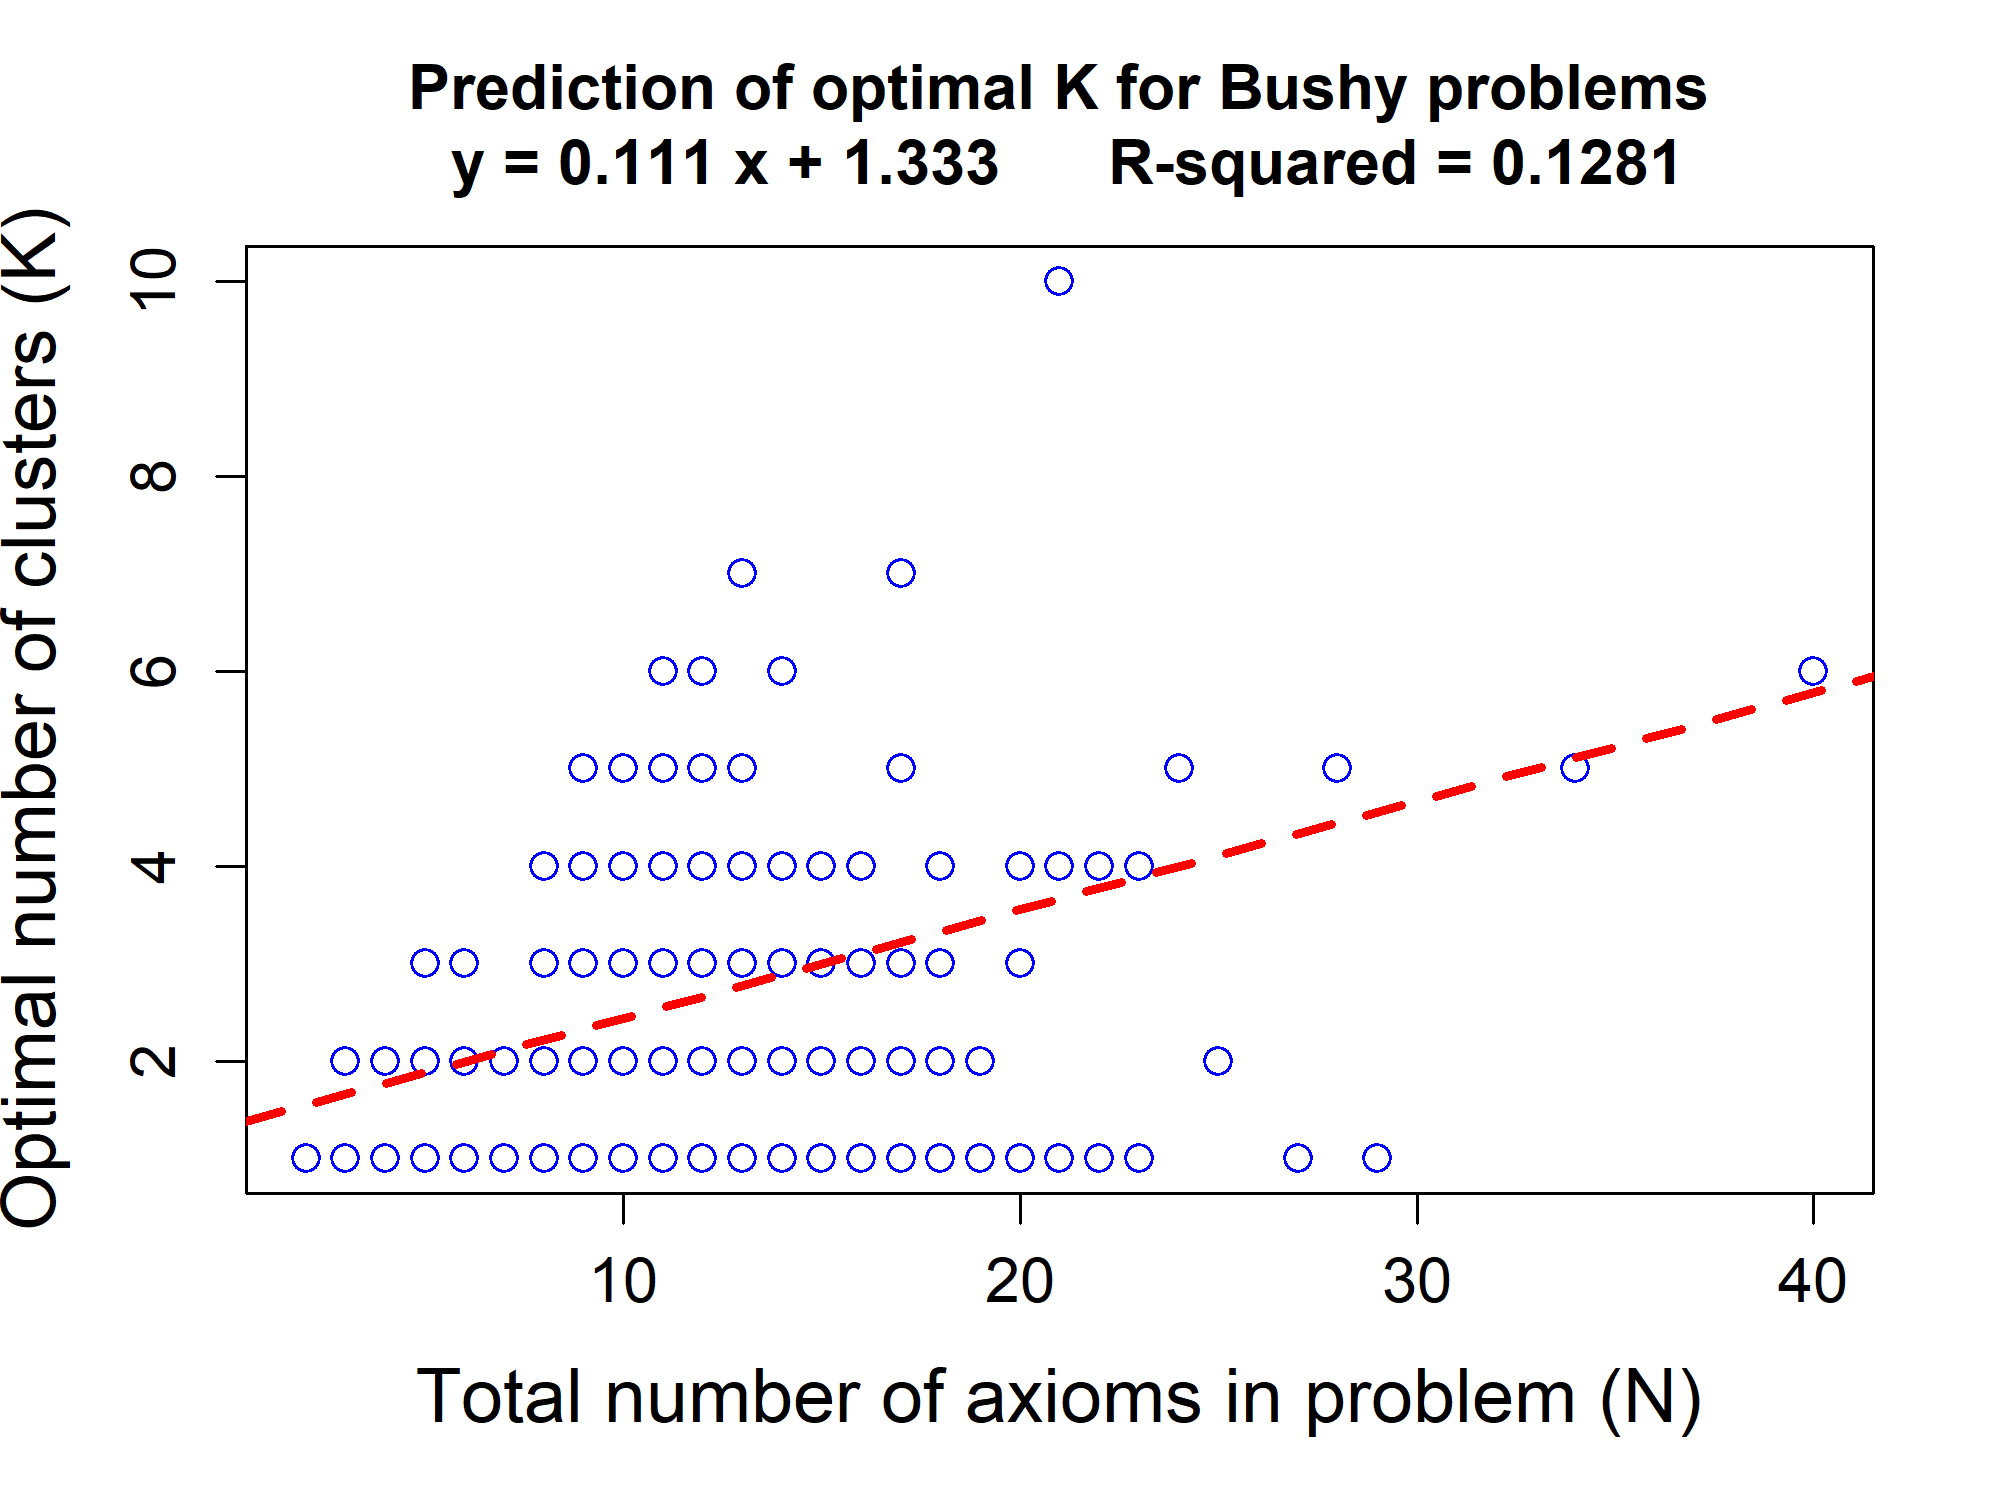
\includegraphics[scale=0.42]{median-regression-optimal-k-bushy-325.png}
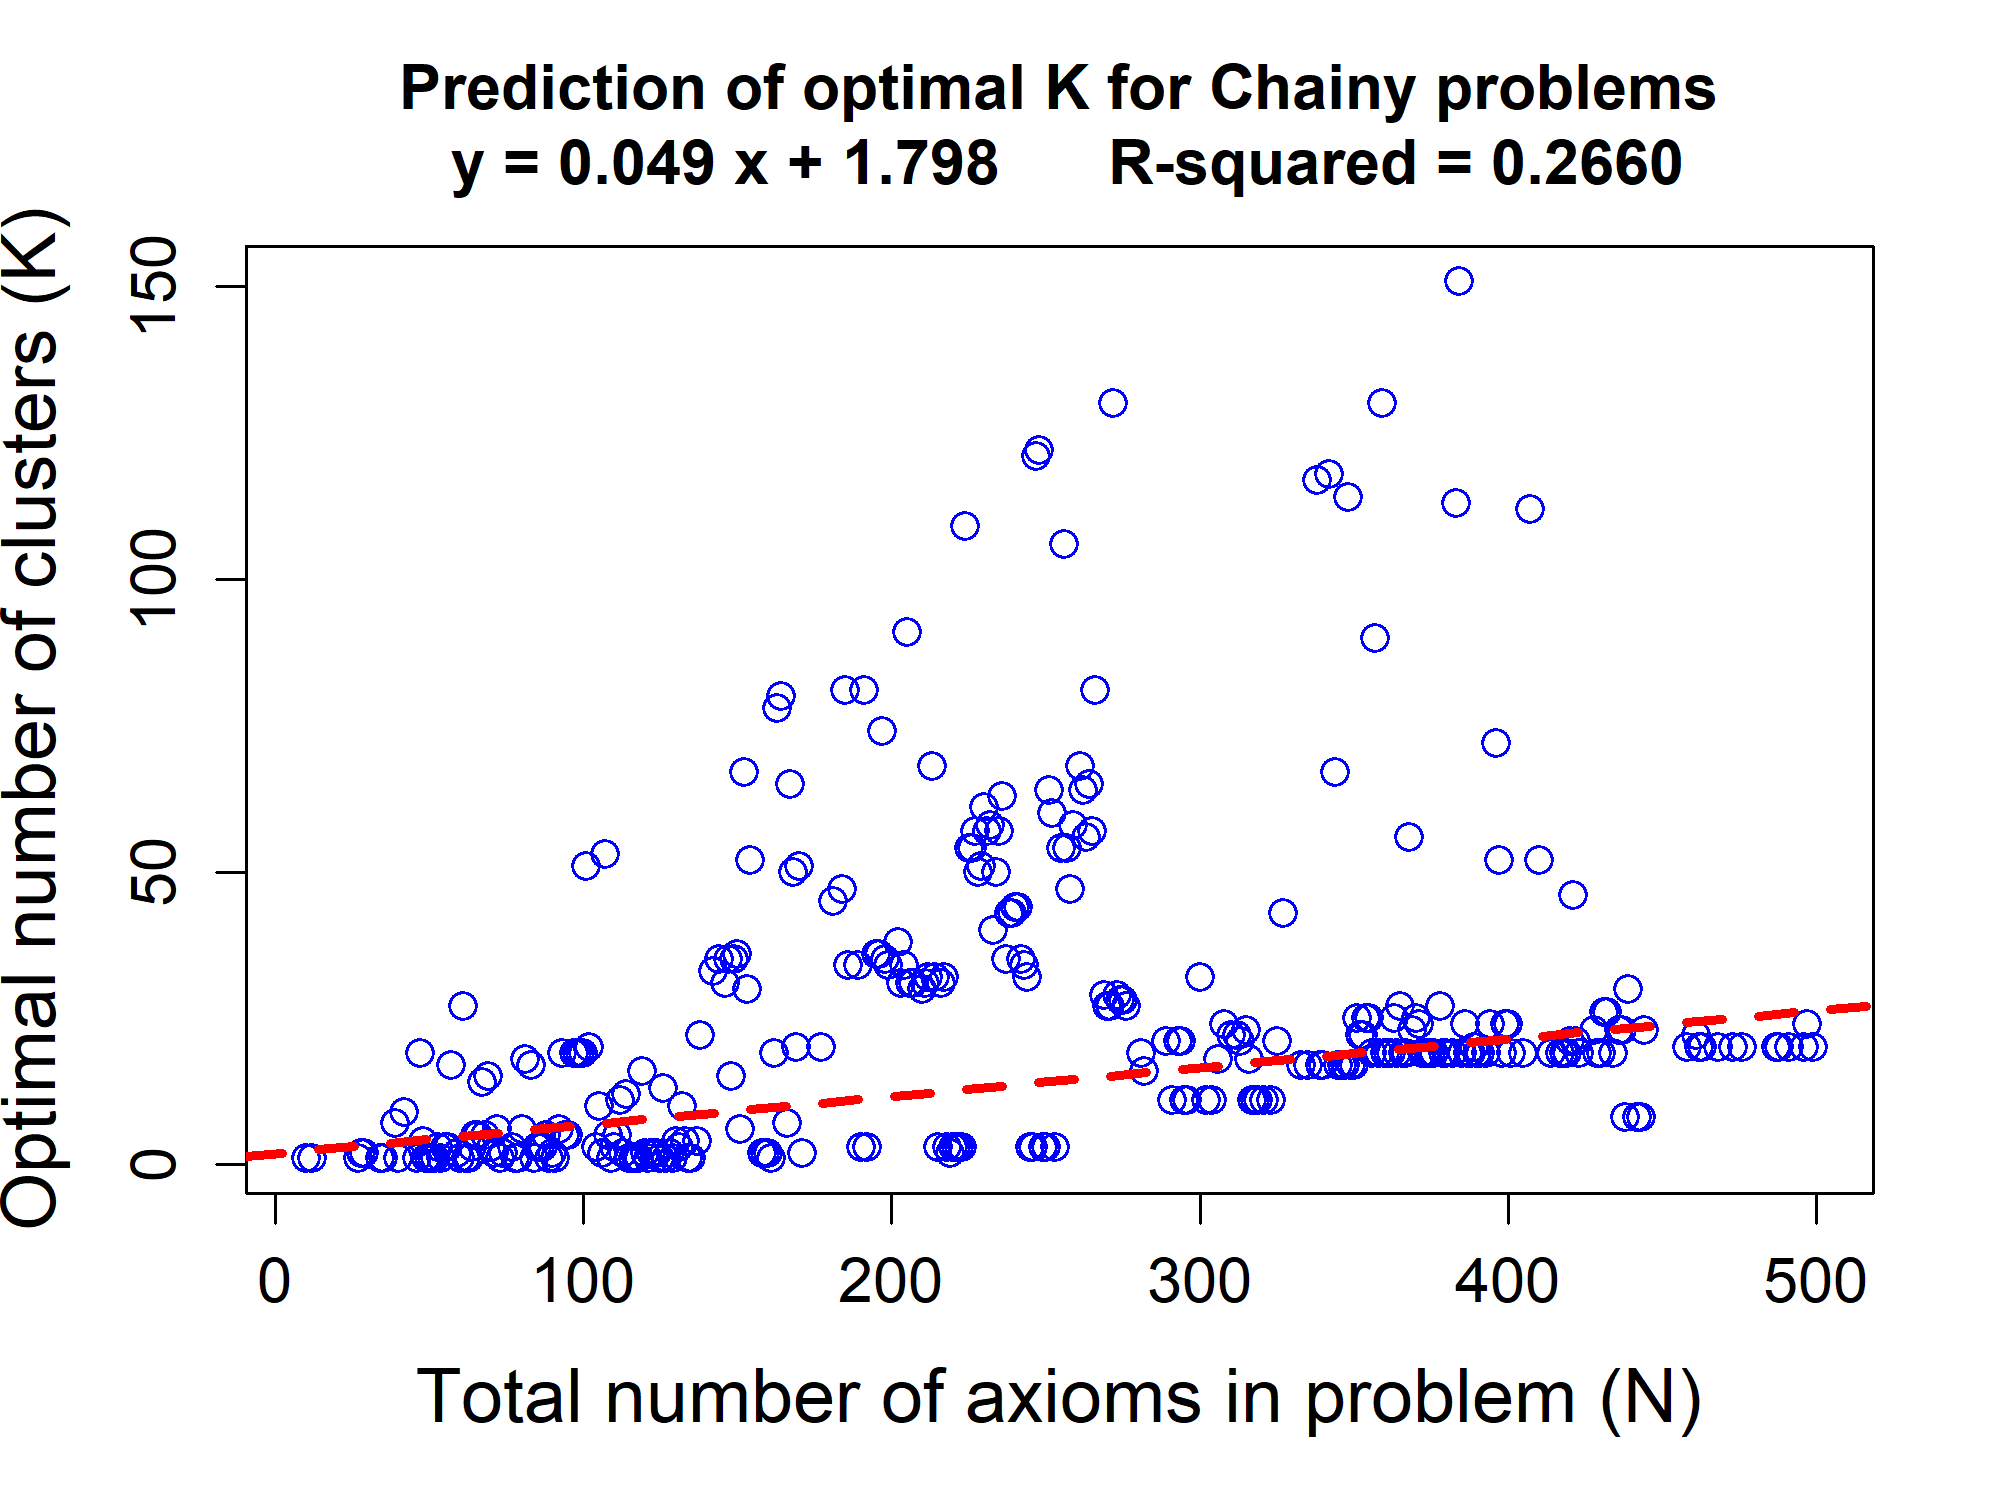
\includegraphics[scale=0.42]{median-regression-optimal-k-chainy-325.png}\\
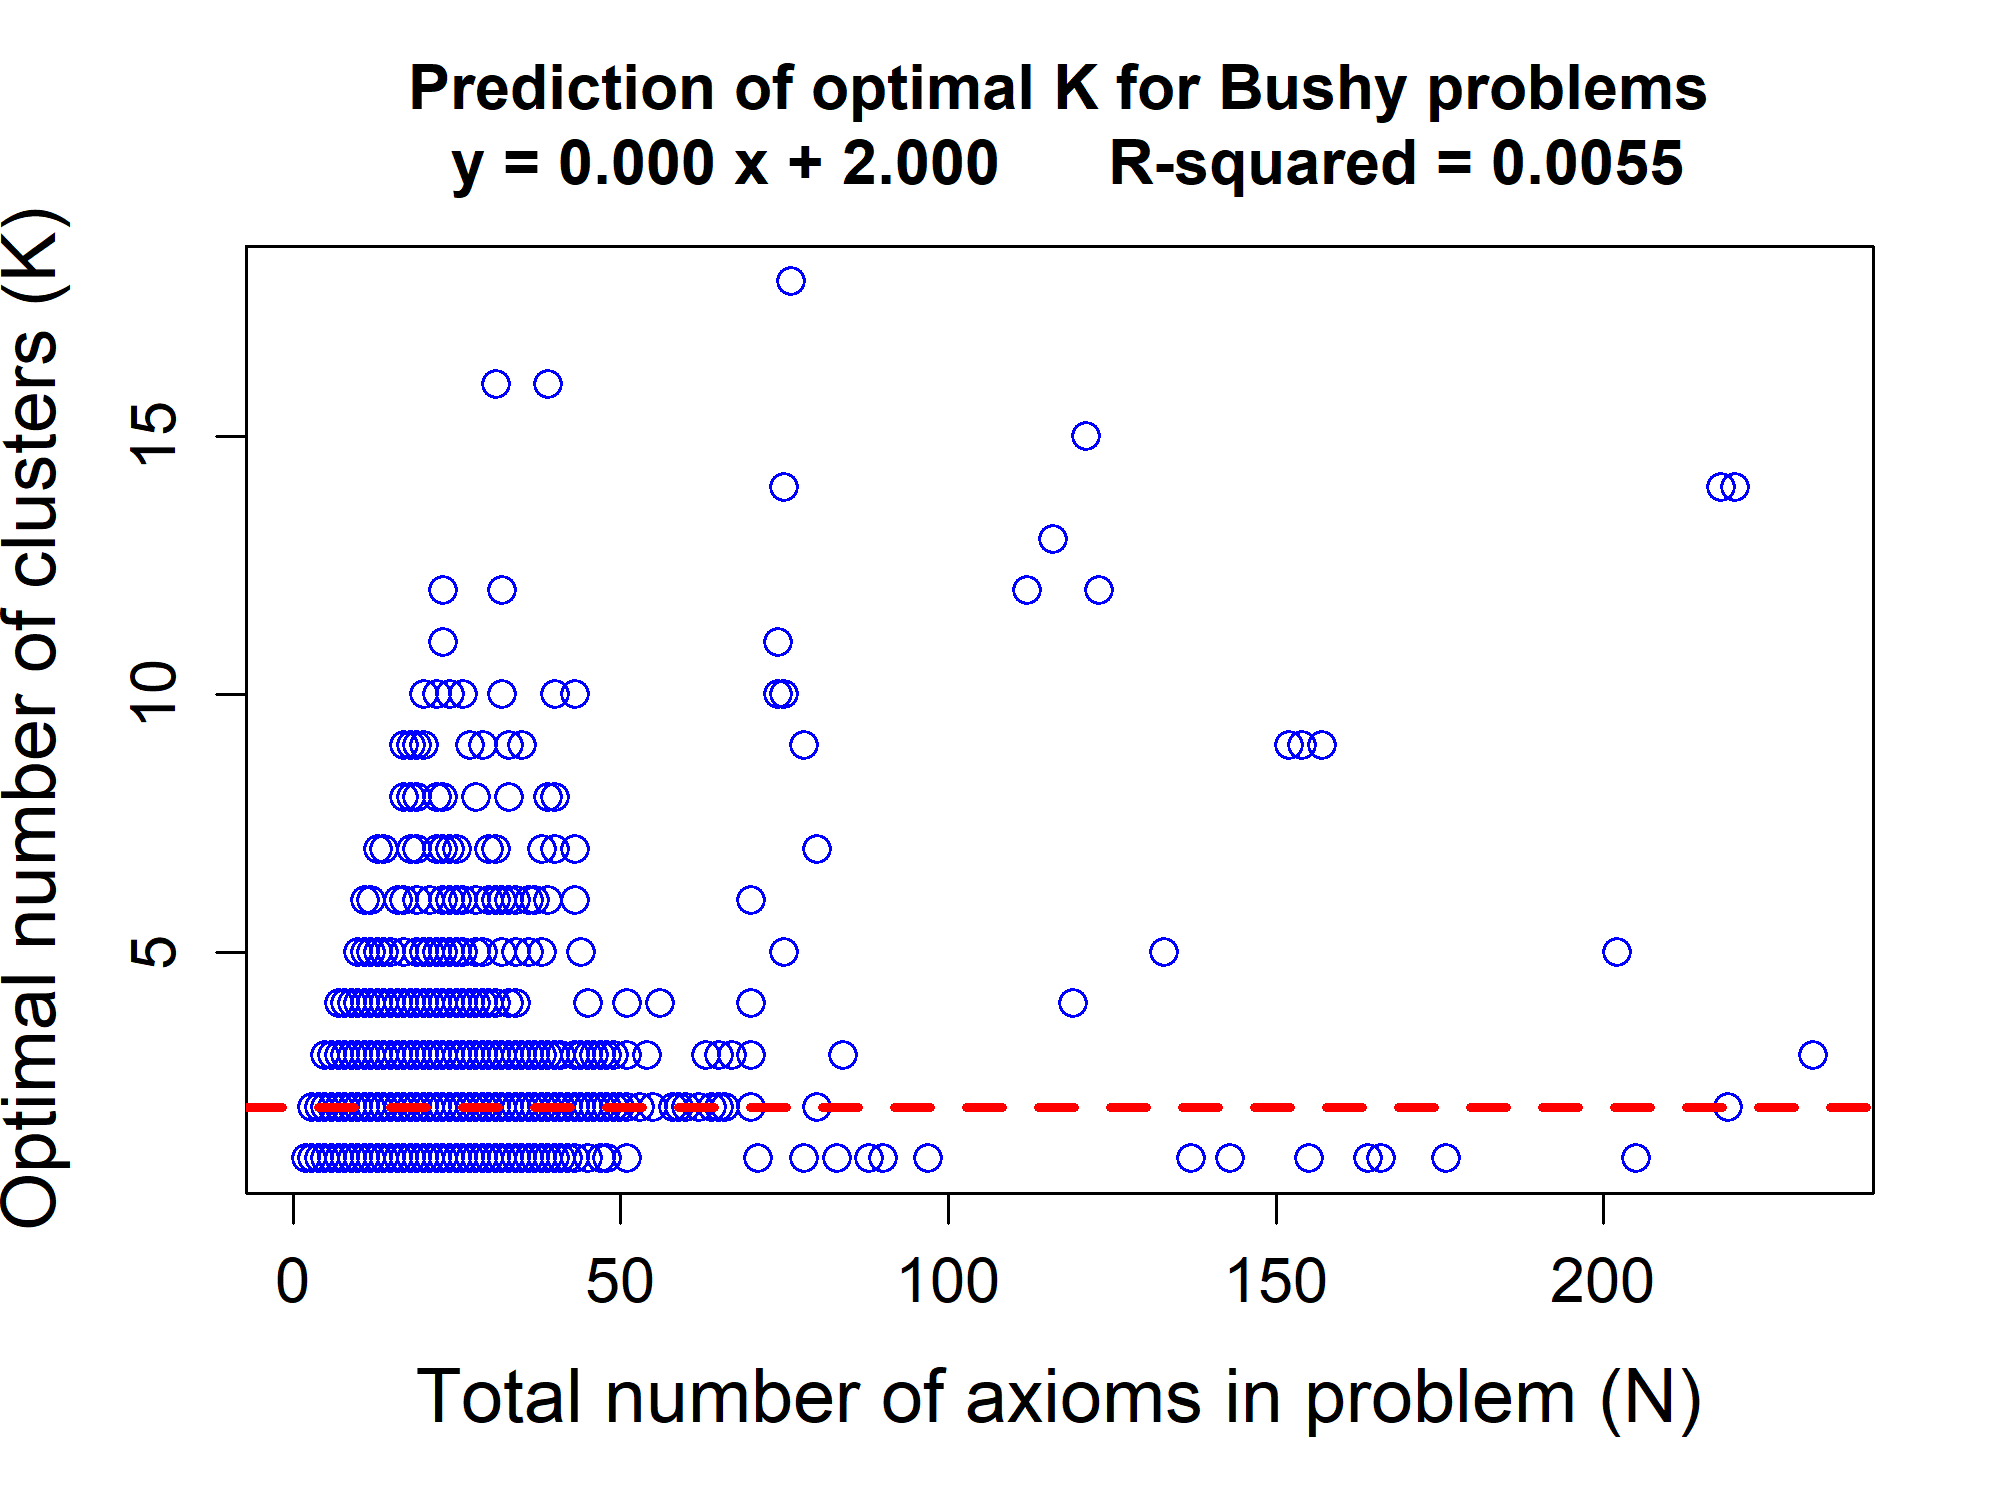
\includegraphics[scale=0.42]{median-regression-optimal-k-bushy-1551.png}
\caption{Best number of clusters vs. Number of formulae}
\label{fig:median-regression}
\end{figure}

%------------------------------------------------------------------------------
\subsection{Greedy Tree plus Nearest Neighbours}
\label{Zihao}

This axiom selection technique views the formulae of a problem as nodes
of a complete undirected graph, with the similarities between the formulae 
as the edge weights.
Figure~\ref{GreedyTree} provides a simple illustrative example, in which
{\sf C} is the conjecture and {\sf A}s are the axioms (the figure
omits edges that do not affect the example).
Starting at the conjecture, a greedy tree is built by iteratively visiting all
the axioms most similar to the current leaves of the tree, until axioms that 
have no similarity (or equivalently, infinite dissimilarity) 
to the conjecture are reached. 
These infinitely dissimilar nodes are ignored.
In Figure~\ref{GreedyTree} the thicker edges are those that are followed,
and the axioms with thicker circles are those at which the tree growth 
stops because they have no similarity to the conjecture.
At that stage the light grey axioms are in the tree.
As a final step, all the unvisited axioms most similar to the axioms in the 
greedy tree are added to the tree.
In Figure~\ref{GreedyTree}, that adds the dark grey axioms to the tree.
The axioms in the tree are selected - those are the non-white axiom in
the Figure~\ref{GreedyTree}..

\begin{figure}[h]
\centering
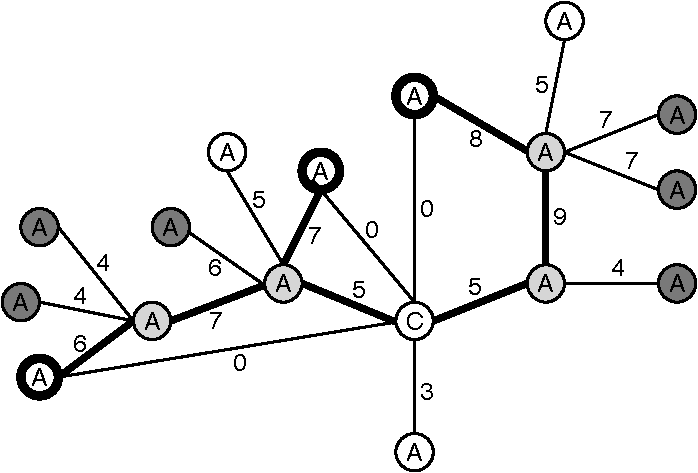
\includegraphics[width=0.5\linewidth]{GreedyTree+NN.pdf}
\caption{A greedy tree}
\label{GreedyTree}
\end{figure}

%------------------------------------------------------------------------------
\section{Evaluation Results}
\label{Results}

The new axiom selection techniques and the axiom selection in the Vampire 
ATP system were evaluated using the metrics.
No particular effort was moade to optimize the implementation of the new
selection techniques; rather, the evaluation aimed to demonstrate the
usefulness of the metrics, and as such no CPU times are presented below.
Two problem sets from each of the bushy and chainy parts of the MPTP2078 
corpus were used. 
The first set was selected by taking the 325 chainy problems with less than 
500 axioms and for which minimally adequate axiom sets of axioms (pruney 
problems) are known, and taking the corresponding 325 bushy problems.
The second set was the 1551 bushy problems and 1369 chainy problems for which
minimally adequate axiom sets (pruney problems) are known.
The smaller set was useful for initial quick testing, and also necessary 
because some of the new techniques could not analyse the chainy problems set 
with the time and computing resources available.

Tables~\ref{Results325} and ~\ref{Results2078} show the results, including
a row for the base case in which all axioms are selected.
The columns are the 
Precision (Prcn), 
Selectivity (Sely), 
Ranking precision (RPrn), 
Ranking density (RDen), 
Adequacy (Adeq),
and the Adequate precision/selectivity/ranking precision/ranking density.

\begin{table}[hbt]
\begin{center}
\begin{tabular}{|l|rrrr|r|rrrr|}
\hline
325 Bushy problems  & \multicolumn{4}{|c|}{Average} & \multicolumn{5}{|c|}{Adequate} \\
Technique       & Prcn & Sely & RPrn & RDen & Adeq & Prcn & Sely & RPrn & RDen \\
\hline
Base            & 0.35 & 1.00 &  -   &  -   & 1.00 & 0.35 & 1.00 &  -   &  -   \\
% E 2.4           & 0.35 & 1.00 &  -   &  -   & 1.00 & 0.35 & 1.00 &  -   &  -   \\
Vampire 4.4     & 0.32 & 0.80 &  -   &  -   & 0.80 & 0.39 & 0.84 &  -   &  -   \\
Q$\infty$       & 0.43 & 0.54 & 0.62 & 0.52 & 0.74 & 0.58 & 0.61 & 0.84 & 0.71 \\
Spectral Cl.    & 0.24 & 0.57 &  -   &  -   & 0.66 & 0.36 & 0.79 &  -   &  -   \\
Greedy Tree+NN  & 0.36 & 0.57 &  -   &  -   & 0.66 & 0.36 & 0.79 &  -   &  -   \\
\hline
\hline
325 Chainy problems & \multicolumn{4}{|c|}{Average} & \multicolumn{5}{|c|}{Adequate} \\
Technique       & Prcn & Sely & RPrn & RDen & Adeq & Prcn & Sely & RPrn & RDen \\
\hline
Base            & 0.06 & 1.00 &  -   &  -   & 1.00 & 0.06 & 1.00 &  -   &  -   \\
% E 2.4           & 0.06 & 1.00 &  -   &  -   & 1.00 & 0.06 & 1.00 &  -   &  -   \\
Vampire 4.4     & 0.08 & 0.55 &  -   &  -   & 0.94 & 0.09 & 0.56 &  -   &  -   \\
Q$\infty$       & 0.08 & 0.53 & 0.57 & 0.21 & 0.85 & 0.09 & 0.56 & 0.67 & 0.25 \\
Spectral Cl.    & 0.05 & 0.48 &  -   &  -   & 0.65 & 0.08 & 0.63 &  -   &  -   \\
Greedy Tree+NN  & 0.05 & 0.79 &  -   &  -   & 0.86 & 0.06 & 0.85 &  -   &  -   \\
\hline
\end{tabular}
\caption{Results for the 325 smaller problems}
\label{Results325}
\end{center}
\end{table}

\begin{table}[hbt]
\begin{center}
\begin{tabular}{|l|rrrr|r|rrrr|}
\hline
1551 Bushy problems  & \multicolumn{4}{|c|}{Average} & \multicolumn{5}{|c|}{Adequate} \\
Technique       & Prcn & Sely & RPrn & RDen & Adeq & Prcn & Sely & RPrn & RDen \\
\hline
Base            & 0.30 & 1.00 &  -   &  -   & 1.00 & 0.30 & 1.00 &  -   &  -   \\
% E 2.4           & 0.30 & 1.00 &  -   &  -   & 1.00 & 0.30 & 1.00 &  -   &  -   \\
Vampire 4.4     & 0.21 & 0.69 &  -   &  -   & 0.58 & 0.35 & 0.76 &  -   &  -   \\
Q$\infty$       & 0.33 & 0.54 & 0.55 & 0.41 & 0.68 & 0.48 & 0.59 & 0.80 & 0.60 \\
Spectral Cl.    & 0.25 & 0.69 &  -   &  -   & 0.76 & 0.33 & 0.83 &  -   &  -   \\
\hline
\hline
1369 Chainy problems & \multicolumn{4}{|c|}{Average} & \multicolumn{5}{|c|}{Adequate} \\
Technique       & Prcn & Sely & RPrn & RDen & Adeq & Prcn & Sely & RPrn & RDen \\
\hline
Base            & 0.02 & 1.00 &  -   &  -   & 1.00 & 0.02 & 1.00 &  -   &  -   \\
% E 2.4           & 0.02 & 0.98 &  -   &  -   & 1.00 & 0.02 & 0.98 &  -   &  -   \\
Vampire 4.4     & 0.03 & 0.40 &  -   &  -   & 0.87 & 0.04 & 0.41 &  -   &  -   \\
Q$\infty$       & 0.03 & 0.53 & 0.46 & 0.07 & 0.81 & 0.04 & 0.56 & 0.56 & 0.09 \\
\hline
\end{tabular}
\caption{Results for all problems with known minimally adequate axiom sets}
\label{Results2078}
\end{center}
\end{table}

For the smaller set of 325 bushy problems Q$\infty$ performs the best, with
the highest precision and lowest selectivity.
It also has a 74\% adequacy.
Moving up to the 325 chainy problems Q$\infty$ and Vampire have the highest
precision, with Q$\infty$ having slightly higher selectivity, and Vampire
better adequacy.
For the 1551 bushy problems Q$\infty$ is again the top performer, now in
terms of precision, selectivity, and adequacy.
Spectral clustering also performs reasonably well, with a better precision
than Vampire, and with the cluster containing the conjecture (recall from 
Section~\ref{Zishi} that two clusters is optimal, and hence used here) 
containing 69\% of the axioms on average.
Finally, for the 1369 chainy problems Q$\infty$ and Vampire again have the 
highest precision, with Vampire having the best selectivity and adequacy.
Overall, Q$\infty$ performs the best on the bushy problems, with Vampire
doing slightly better on the chainy problems.
It is surprising that the very simple Q$\infty$ technique performs 
as well as it does, when compared to the mature (and more complex) Vampire 
selection technique.

The adequacy numbers have to be viewed carefully - it is easy to get an
optimal adequacy simply by selecting all axioms and thus having pessimal
selectivity.
It is interesting to contrast the average and adequate precision values.
The average precision for the base case is better than that of some of the
selection techniques because of the zero precision assigned when an inadequate
set of axioms is selected.
An adequate precision close to the base case, as for, e.g., Spectral 
Clustering and Greedy Tree+NN on both sets of 325 problems,
indicates that doing the axiom selection is probably wasted effort.

There is a correlation, but not a particularly strong correlation, between 
the number of axioms in a problem and the precision of the Vampire and 
Q$\infty$ axiom selections, e.g., around 40\% for the chainy problems.
This suggests that the axiom selection techniques might scale well to
larger problems.

Overall, the precision values are disappointingly low, especially for the
chainy problems.
For Q$\infty$ the ranking density is similarly low, so that even with perfect
ranking precision the raw precision cannot be very good.
Figure~\ref{fig:PrcnChainy} shows the distributions of the precision values
for the chainy problems.
In each plot the left set of points are for those problems where an adequate
set of axioms was selected, and the right set of point are for those problems
where an inadequate set of axioms was selected.
For the majority of problems the precision in less that 0.1, i.e., less than
10\% of selected axioms are used in a proof.

\begin{figure}[h]
\centering
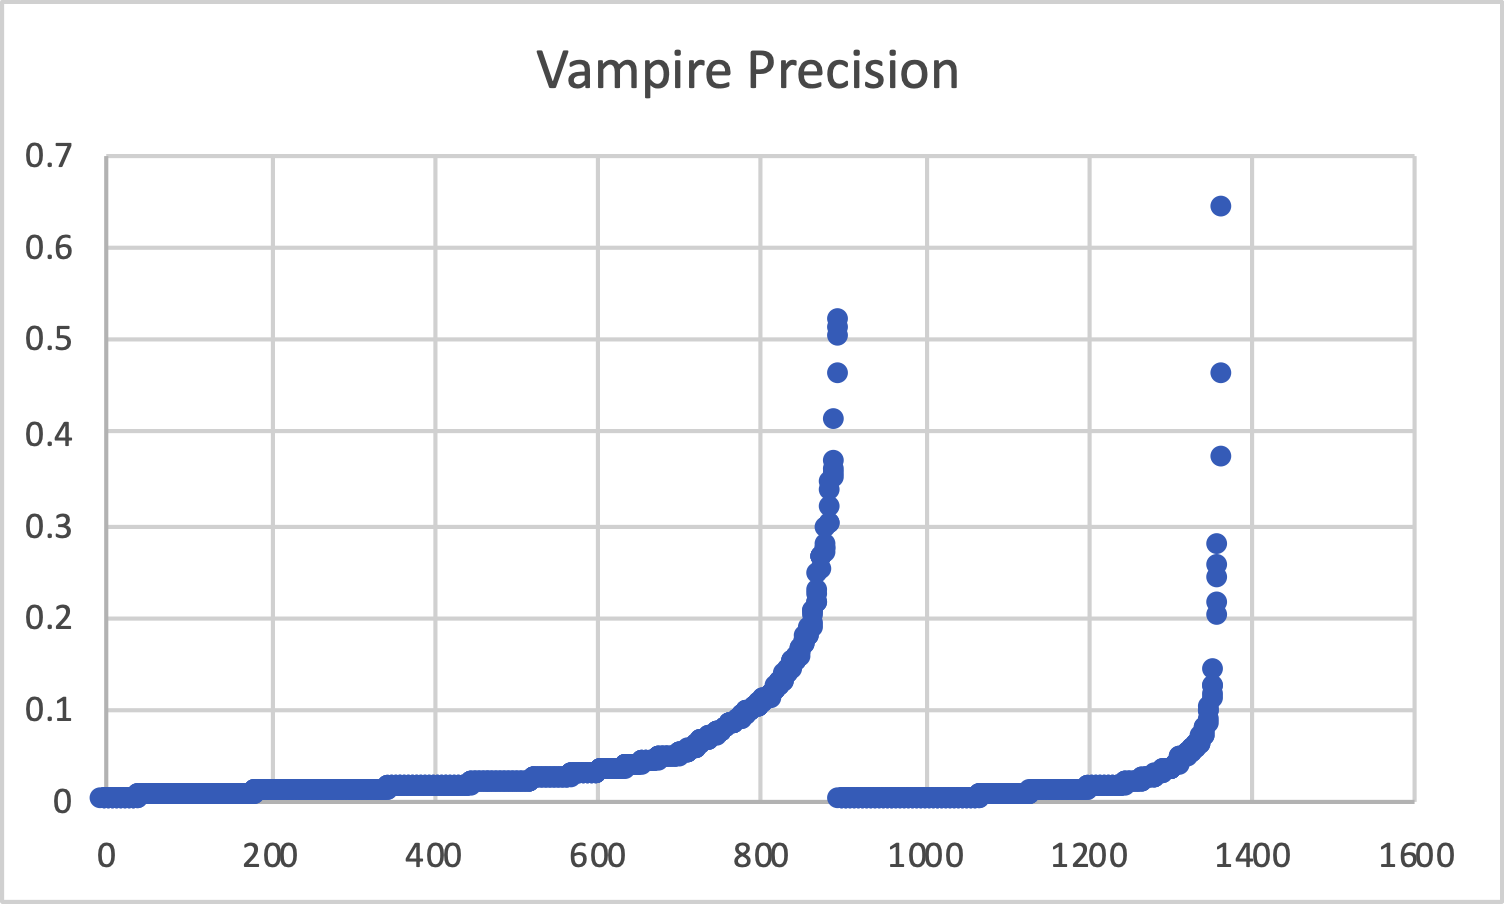
\includegraphics[width=0.45\textwidth]{PrcnChainyVampire.png}~~~~
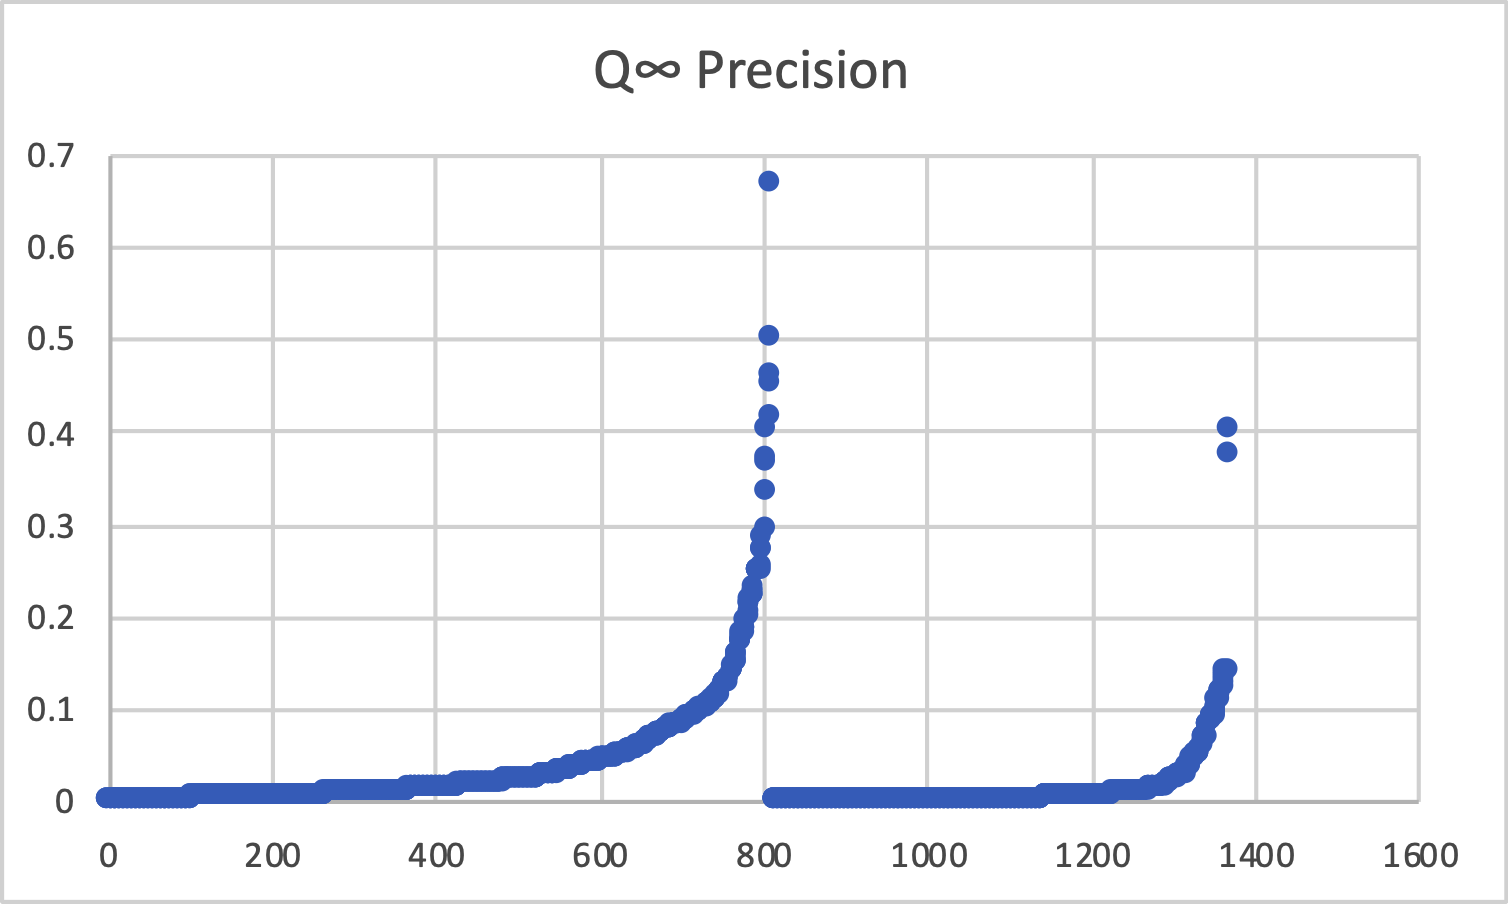
\includegraphics[width=0.45\textwidth]{PrcnChainyQinf.png}
\caption{Distribution of precision values for chainy problems}
\label{fig:PrcnChainy}
\end{figure}

%------------------------------------------------------------------------------
\subsection{Evaluating the Metrics}
\label{EvaluationOfMetrics}

As was noted in the introduction to this paper, while metrics such as
those presented in this paper are useful for quick evaluation of axiom
selection techniques, the ``proof is in the pudding''.
The quality of the metrics needs to be established by comparing them with 
eventual ATP system performance.
An initial evaluation of the precision metric has been performed by using
the Vampire and Q$\infty$ axiom selections, and looking at the performance 
of E on the resultant reduced problems.
This was done for the 1551 bushy problems and 1369 chainy problems for
which there are known minimally adequate axiom sets, so that the precision 
could be computed.
The testing was done with a 300s CPU time limit on 
computers with a dual-core Intel(R) Xeon(R) E5-2609 2.50GHz CPU,
8GB memory, and running the CentOS Linux release 7.6.1810 operating system.
The results are shown in Table~\ref{EvaluationOfMetrics}.

In all four cases the precision of the unsolved problems is much lower than for 
the solved problems - the precision metric aligns correctly with the solvability 
of the reduced problems.
The numbers of problems with precision 0.00 and 1.00 also align with the numbers
of solutions, with higher numbers of solved problems with precision 1.00, and
higher numbers of unsolved problems with precision 0.00.
Overall, these results indicate that the precision metric does correctly
evaluate the quality of the axiom selection.

The attentive reader might have noticed that there are some solved problems with
precision 0.00, which is weird because the precision should be 0.00 only if the 
selected axioms are not an adequate set (Section~\ref{TheMetrics}).
This indicates that these experiments revealed some new minimally adequate 
sets of axioms for some problems in the MPTP2078 corpus, and thus that some 
further pruney problems need to be created.

\begin{table}[hbt]
\begin{center}
\begin{tabular}{|l|rr|rr|rr|rr|}
\hline
1551 Bushy      & \multicolumn{4}{|c|}{Vampire selection} & \multicolumn{4}{|c|}{Q$\infty$ selection} \\
problems        & \multicolumn{2}{|c|}{Solved} & \multicolumn{2}{|c|}{Unsolved} & \multicolumn{2}{|c|}{Solved} & \multicolumn{2}{|c|}{Unsolved} \\
\hline
\# Problems     &  848 & (55\%) &  703 & (45\%) &  969 & (62\%) &  582 & (38\%) \\
Avg Prcn        & 0.35 &        & 0.03 &        & 0.48 &        & 0.07 &        \\
\# Prcn 0.00    &    5 & (~1\%) &  646 & (92\%) &    3 & (~0\%) &  487 & (84\%) \\
\# Prcn 1.00    &    7 & (~1\%) &    0 & (~0\%) &   63 & (~7\%) &    0 & (~0\%) \\
\hline
\hline
1369 Chainy     & \multicolumn{4}{|c|}{Vampire selection} & \multicolumn{4}{|c|}{Q$\infty$ selection} \\
problems        & \multicolumn{2}{|c|}{Solved} & \multicolumn{2}{|c|}{Unsolved} & \multicolumn{2}{|c|}{Solved} & \multicolumn{2}{|c|}{Unolved} \\
\hline
\# Problems     &  901 & (66\%) &  468 & (34\%) &  812 & (59\%) &  557 & (41\%) \\
Avg Prcn        & 0.04 &        & 0.02 &        & 0.04 &        & 0.01 &        \\
\# Prcn 0.00    &   19 & (~2\%) &  159 & (34\%) &   11 & (~1\%) &  243 & (44\%) \\
\# Prcn 1.00    &    0 & (~0\%) &    0 & (~0\%) &    0 & (~0\%) &    0 & (~0\%) \\
\hline
\end{tabular}
\caption{Evaluation of Vampire and Q$\infty$ axiom selection wrt E}
\label{EvaluationOfMetrics}
\end{center}
\end{table}

%------------------------------------------------------------------------------
\section{Conclusion}
\label{Conclusion}

The main contribution of this paper is metrics for evaluating axiom selection 
techniques without having to run an ATP system on the reduced problems.
Three new axiom selection techniques have also been presented.
Results from evaluating the new techniques and the axiom selection in the 
Vampire ATP system have been presented.

Future work includes a more comprehensive evaluation of the metrics, to
confirm that the metrics do provide a meaningful evaluation of the axiom
selection techniques.
It will also be interesting to apply the metrics to the axiom selection
techniques found in other ATP systems such as E, GKC \cite{Tam19},
iProver \cite{Kor08}, Leo-III \cite{SB18}, and MaLARea.

The results show that there is lots of room for further research and 
improvement in axiom selection.
We are currently investigating the use of network propagation \cite{SY07}, 
adopted from the analysis of protein-protein interaction networks
\cite{DD+20}, for analysing the formula similarity graphs.  
One interesting possibility is pipelining axiom selection tools so that
the first in the pipeline receives the original problem, it's output
becomes the input to the second in the pipeline, and so on.
Finally, the three new axiom selection techniques all build on the
dissimilarity and similarity measures described in 
Section~\ref{QinghuaDistance}.
Further development and improvement of those measures, or their complete
replacement, would have consequential impacts downstream.

%------------------------------------------------------------------------------
\label{sect:bib}
\bibliographystyle{plain}
\bibliography{Bibliography}
%------------------------------------------------------------------------------
\end{document}
%------------------------------------------------------------------------------

